\section{Q4 Bonus: Kernel SVMs, Margin Geometry, and Clustering}
\label{sec:q4}

\subsection{Q4(a): Systematic SVM Parameter and Kernel Sweep}
\paragraph{Experimental Protocol and Representation Space.}
To evaluate kernel methods on deep representations, we utilize the frozen 64-dimensional penultimate representation extracted from our trained FairCNN model from Q2(a) (verified at $\mathbf{72.05\%}$ test accuracy). We use the fixed, stratified $5{,}000$-sample training subset $\mathcal{D}_{\text{svm}}$ ($500$ samples per class). Preprocessing via \texttt{StandardScaler} is fitted strictly on the $5{,}000$ training representations and applied frozen to the validation and test splits.

We execute an exhaustive $15$-configuration grid sweep spanning three kernel families and five regularization parameters:
\begin{equation}
\begin{aligned}
    \mathcal{K} &\in \{\text{Linear}, \text{RBF}, \text{Poly} (d=3)\}, \\
    C &\in \{0.01, 0.1, 1.0, 10.0, 100.0\}.
\end{aligned}
\end{equation}

\begin{table}[t]
\centering
\caption{Q4(a) Exhaustive 15-Configuration SVM Grid Sweep on 64-D FairCNN representations. Model selection was conducted strictly using validation accuracy on the full $5{,}000$-sample validation set.}
\label{tab:q4a_sweep}
\resizebox{\columnwidth}{!}{
\begin{tabular}{lccccc}
\toprule
\textbf{Kernel} & \textbf{Reg. $C$} & \textbf{Train Acc} & \textbf{Val Acc ($N=5\text{k}$)} & \textbf{SVs ($N_{\text{SV}}$)} & \textbf{SV Frac ($\rho_{\text{SV}}$)} \\
\midrule
Linear & $0.01$  & $95.32\%$ & $72.84\%$ & $2{,}018$ & $40.36\%$ \\
Linear & $0.1$   & $95.76\%$ & $72.18\%$ & $1{,}118$ & $22.36\%$ \\
Linear & $1.0$   & $96.88\%$ & $71.50\%$ & $875$     & $17.50\%$ \\
Linear & $10.0$  & $97.80\%$ & $70.54\%$ & $854$     & $17.08\%$ \\
Linear & $100.0$ & $98.52\%$ & $69.98\%$ & $844$     & $16.88\%$ \\
\midrule
RBF    & $0.01$  & $91.40\%$ & $72.22\%$ & $4{,}828$ & $96.56\%$ \\
\textbf{RBF} & $\mathbf{0.1}$ & $\mathbf{94.74\%}$ & $\mathbf{72.88\%}$ & $\mathbf{3{,}124}$ & $\mathbf{62.48\%}$ \\
RBF    & $1.0$   & $96.28\%$ & $72.52\%$ & $1{,}788$ & $35.76\%$ \\
RBF    & $10.0$  & $98.32\%$ & $71.92\%$ & $1{,}343$ & $26.86\%$ \\
RBF    & $100.0$ & $99.90\%$ & $71.76\%$ & $1{,}374$ & $27.48\%$ \\
\midrule
Poly ($d=3$) & $0.01$  & $62.32\%$ & $52.38\%$ & $4{,}324$ & $86.48\%$ \\
Poly ($d=3$) & $0.1$   & $84.54\%$ & $67.02\%$ & $2{,}983$ & $59.66\%$ \\
Poly ($d=3$) & $1.0$   & $93.36\%$ & $71.18\%$ & $1{,}840$ & $36.80\%$ \\
Poly ($d=3$) & $10.0$  & $97.26\%$ & $71.42\%$ & $1219$    & $24.38\%$ \\
Poly ($d=3$) & $100.0$ & $99.48\%$ & $70.58\%$ & $1141$    & $22.82\%$ \\
\bottomrule
\end{tabular}
}
\end{table}

\begin{figure}[t]
\centering
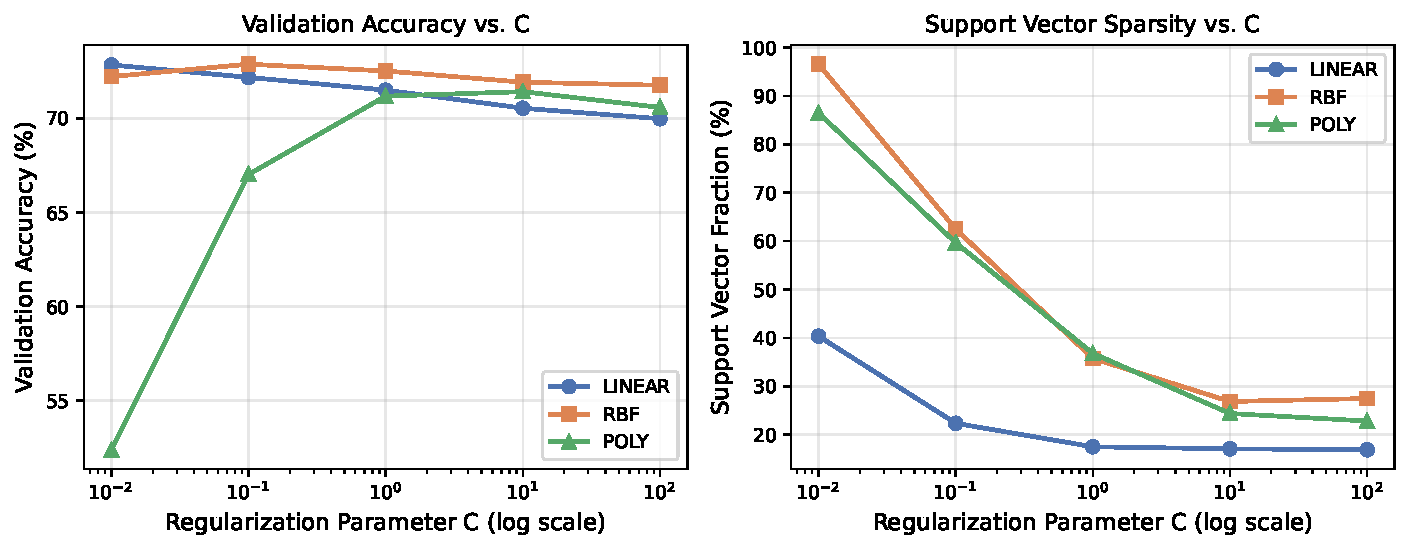
\includegraphics[width=0.78\linewidth]{figures/q4a_svm_sweep.pdf}
\caption{Q4(a) Validation accuracy (left) and support vector fraction (right) as a function of regularization parameter $C$ across Linear, RBF, and Polynomial kernels.}
\label{fig:q4a_sweep}
\end{figure}

\paragraph{Validation-Based Model Selection and Test Result.}
As documented in Table~\ref{tab:q4a_sweep} and Figure~\ref{fig:q4a_sweep}, the **RBF Kernel with $C = 0.1$** achieved the highest accuracy on the full $5{,}000$-sample validation set ($\mathbf{72.88\%}$), with a support vector fraction of $\rho_{\text{SV}} = 62.48\%$ ($3{,}124$ SVs). 

At lower regularization ($C=0.01$), the RBF margin is overly soft, causing nearly all samples to act as support vectors ($\rho_{\text{SV}} = 96.56\%$). At higher regularization ($C \ge 1.0$), the dual solver penalizes margin violations severely, driving training accuracy to $99.90\%$ but inducing validation degradation ($71.76\%$). 

Following selection, the locked model was evaluated strictly once on the official test set:
\begin{equation}
    \text{Official Test Accuracy} = \mathbf{71.64\%}.
\end{equation}
Remarkably, an RBF SVM trained on only $5{,}000$ samples over frozen 64-D CNN features achieves $71.64\%$ accuracy—matching the full end-to-end FairCNN classifier ($72.05\%$) within $0.41\%$.

\begin{figure*}[t]
\centering
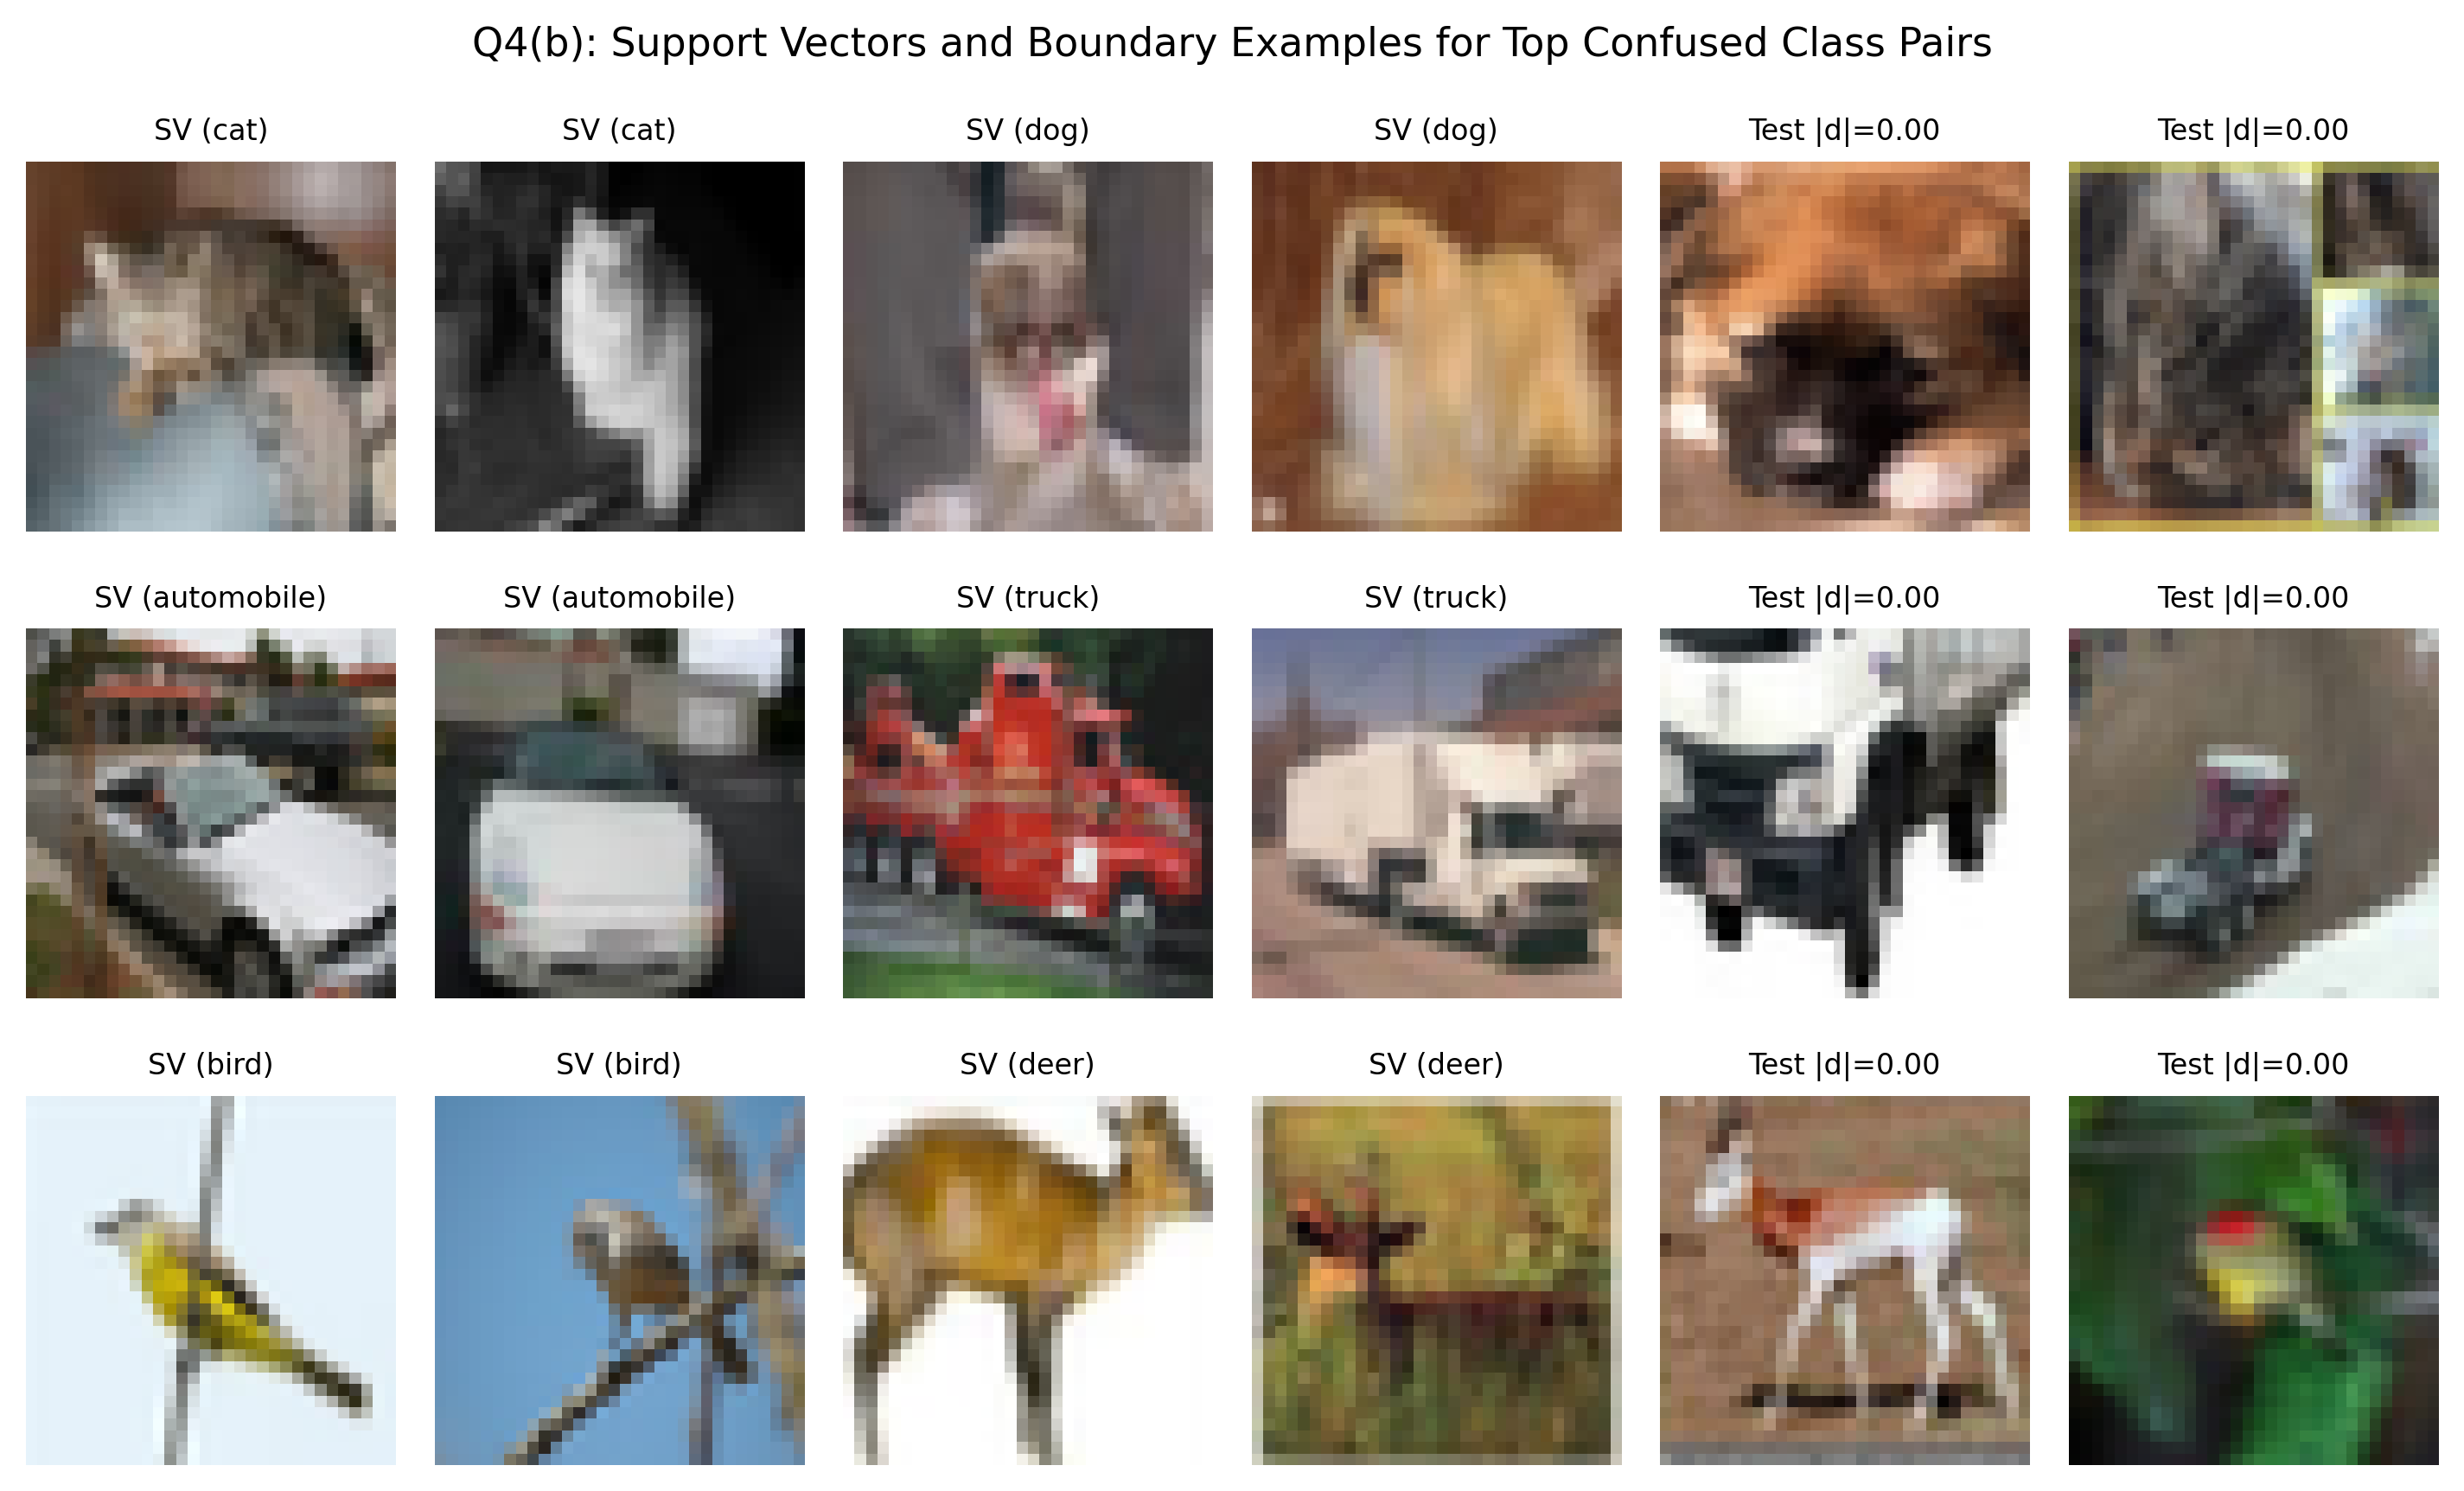
\includegraphics[width=0.88\textwidth]{figures/q4b_hard_pairs.png}
\caption{Q4(b) Boundary geometry visualization for the top-3 difficult class pairs: Training Support Vectors for Class A (cols 1--2), Training Support Vectors for Class B (cols 3--4), and Closest Test Samples near the pairwise boundary (cols 5--6) annotated with their raw One-vs-One boundary-proximity scores $|f_{i,j}(\mathbf{x})|$.}
\label{fig:q4b_hard_pairs}
\end{figure*}

\subsection{Q4(b): Hard Class-Pair Decision Boundary Geometry}
\paragraph{Identification of Difficult Pairs.}
Using the post-selection test confusion matrix of the selected RBF SVM, the three most confused class pairs were identified:
\begin{enumerate}
    \item \textbf{Cat vs. Dog:} $391$ total symmetric errors ($208$ cats misclassified as dogs; $183$ dogs misclassified as cats).
    \item \textbf{Automobile vs. Truck:} $181$ total symmetric errors ($98$ autos as trucks; $83$ trucks as autos).
    \item \textbf{Bird vs. Deer:} $171$ total symmetric errors ($81$ birds as deer; $90$ deer as birds).
\end{enumerate}

\paragraph{Raw One-vs-One Boundary-Proximity Formulation.}
To rigorously locate samples near the decision boundary, we evaluate the raw pairwise One-vs-One (OVO) decision scores:
\begin{equation}
    f_{i,j}(\mathbf{x}) = \sum_{k \in \text{SV}_{i,j}} y_k \alpha_k K(\mathbf{x}_k, \mathbf{x}) + b_{i,j}.
\end{equation}
We emphasize a key theoretical distinction: for non-linear kernels like RBF, $|f_{i,j}(\mathbf{x})|$ is an unnormalized \textbf{boundary-proximity score} rather than a Euclidean geometric distance in input space, because the mapping $\Phi(\mathbf{x})$ into reproducing kernel Hilbert space (RKHS) curves the metric. The exact separating hyperplane corresponds to $f_{i,j}(\mathbf{x}) = 0$, and the margin boundaries lie at $f_{i,j}(\mathbf{x}) = \pm 1$.

\begin{table}[t]
\centering
\caption{Q4(b) Dual Support Vector Counts and Closest Test Sample Boundary-Proximity Scores for the Top-3 Difficult Class Pairs.}
\label{tab:q4b_geometry}
\resizebox{\columnwidth}{!}{
\begin{tabular}{lcccc}
\toprule
\textbf{Difficult Pair} & \textbf{Pair Errors} & \textbf{Class A SVs} & \textbf{Class B SVs} & \textbf{Closest Test Scores $|f_{i,j}(\mathbf{x})|$} \\
\midrule
Cat vs. Dog   & $391$ & $432$ ($86.4\%$) & $380$ ($76.0\%$) & $[0.0004, 0.0013, 0.0029, 0.0037]$ \\
Auto vs. Truck & $181$ & $243$ ($48.6\%$) & $246$ ($49.2\%$) & $[0.0006, 0.0021, 0.0039, 0.0055]$ \\
Bird vs. Deer & $171$ & $373$ ($74.6\%$) & $345$ ($69.0\%$) & $[0.0007, 0.0015, 0.0029, 0.0030]$ \\
\bottomrule
\end{tabular}
}
\end{table}

\paragraph{Geometric and Morphological Analysis.}
As documented in Table~\ref{tab:q4b_geometry} and Figure~\ref{fig:q4b_hard_pairs}:
\begin{itemize}
    \item \textbf{Cat vs. Dog (Extreme Manifold Tangency):} Over $80\%$ of training examples for both classes serve as support vectors ($432$ cat SVs, $380$ dog SVs). The closest test samples lie virtually on the decision boundary ($|f_{3,5}| \le 0.0037 \ll 1.0$). Both classes share quadruped morphology, domestic scene contexts, and similar ear/fur textures, producing severe manifold tangency in 64-D space.
    \item \textbf{Automobile vs. Truck (Geometric Box Silhouette):} Fewer support vectors are recruited ($\sim 49\%$), with errors heavily concentrated on box-profile vehicles (SUVs, vans, pickup trucks) where flat-bed geometry overlaps with passenger car silhouettes.
    \item \textbf{Bird vs. Deer (Contextual Foliage Bias):} In outdoor wildlife images, shared natural green vegetation and forest backgrounds cause convolutional texture representations to cluster adjacently, requiring high support vector density ($74.6\%$ and $69.0\%$) to construct a nonlinear separating boundary.
\end{itemize}

\begin{table}[!htbp]
\centering
\caption{Q4(c) Train-Only Label-Free Clustering Model Selection across candidate cluster counts $K$ on $5{,}000$ training representations.}
\label{tab:q4c_selection}
\resizebox{\columnwidth}{!}{
\begin{tabular}{ccccc}
\toprule
\textbf{Clusters $K$} & \textbf{K-Means Inertia ($\downarrow$)} & \textbf{Silhouette ($\uparrow$)} & \textbf{GMM BIC ($\downarrow$)} & \textbf{GMM AIC ($\downarrow$)} \\
\midrule
$6$  & $136{,}526.9$ & $\mathbf{0.1933}$ & $177{,}493.7$ & $172{,}455.9$ \\
$8$  & $121{,}791.7$ & $0.1779$ & $153{,}461.2$ & $146{,}741.9$ \\
$\mathbf{10}$ & $\mathbf{113{,}816.3}$ & $0.1632$ & $138{,}307.6$ & $129{,}907.0$ \\
$12$ & $109{,}659.8$ & $0.1463$ & $120{,}570.3$ & $110{,}488.2$ \\
$14$ & $106{,}364.5$ & $0.1341$ & $\mathbf{116{,}214.9}$ & $\mathbf{104{,}451.4}$ \\
\bottomrule
\end{tabular}
}
\end{table}

\subsection{Q4(c): Unsupervised Clustering vs. Supervised SVM}
\paragraph{Train-Only Label-Free Model Selection.}
To determine clustering hyperparameters without label leakage, we evaluated K-Means and Gaussian Mixture Models (GMM, diagonal covariance) across $K \in \{6, 8, 10, 12, 14\}$ strictly on the $5{,}000$ training representations without labels (Table~\ref{tab:q4c_selection}).

\noindent\textbf{Criteria Trade-Off:} Silhouette score peaks at $K=6$ ($0.1933$) and gradually declines ($0.1632$ at $K=10$, $0.1341$ at $K=14$). Conversely, training inertia drops steeply from $K=6$ to $K=10$ ($\Delta = -16.6\%$) before flattening ($\Delta = -3.6\%$ from $K=10$ to $K=12$). BIC and AIC trend downward with component capacity.

\noindent\textbf{Pragmatic Selection:} We transparently acknowledge that $K=10$ represents a \textit{pragmatic elbow choice} balancing within-cluster compactness against over-fragmentation, rather than a point unanimously favored by every criterion.

\begin{table}[t]
\centering
\caption{Q4(c) Recomputed and Verified Test Contingency Table for Unsupervised K-Means ($K=10$) across all $10{,}000$ official CIFAR-10 test samples. Every row and column sum is explicitly validated: $\sum_{i,j} C_{i,j} = 10{,}000$.}
\label{tab:q4c_contingency_full}
\resizebox{\columnwidth}{!}{
\begin{tabular}{lccccccccccc}
\toprule
\textbf{Cluster ID} & \textbf{Airplane} & \textbf{Automobile} & \textbf{Bird} & \textbf{Cat} & \textbf{Deer} & \textbf{Dog} & \textbf{Frog} & \textbf{Horse} & \textbf{Ship} & \textbf{Truck} & \textbf{Row Total} \\
\midrule
Cluster 0 & $19$  & $\mathbf{820}$ & $2$   & $5$   & $3$   & $3$   & $5$   & $1$   & $24$  & $82$  & $964$ \\
Cluster 1 & $31$  & $18$  & $94$  & $\mathbf{535}$ & $74$  & $279$ & $104$ & $58$  & $30$  & $31$  & $1{,}254$ \\
Cluster 2 & $113$ & $2$   & $\mathbf{579}$ & $83$  & $82$  & $42$  & $56$  & $46$  & $9$   & $6$   & $1{,}018$ \\
Cluster 3 & $\mathbf{703}$ & $37$  & $74$  & $17$  & $28$  & $7$   & $9$   & $32$  & $86$  & $40$  & $1{,}033$ \\
Cluster 4 & $36$  & $97$  & $3$   & $10$  & $2$   & $2$   & $1$   & $14$  & $22$  & $\mathbf{799}$ & $986$ \\
Cluster 5 & $69$  & $18$  & $2$   & $12$  & $2$   & $3$   & $3$   & $1$   & $\mathbf{814}$ & $23$  & $947$ \\
Cluster 6 & $6$   & $5$   & $81$  & $73$  & $69$  & $15$  & $\mathbf{762}$ & $5$   & $6$   & $3$   & $1{,}025$ \\
Cluster 7 & $13$  & $2$   & $24$  & $15$  & $81$  & $35$  & $1$   & $\mathbf{682}$ & $2$   & $10$  & $865$ \\
Cluster 8 & $3$   & $0$   & $28$  & $181$ & $18$  & $\mathbf{537}$ & $10$  & $84$  & $2$   & $1$   & $864$ \\
Cluster 9 & $7$   & $1$   & $113$ & $69$  & $\mathbf{641}$ & $37$  & $49$  & $77$  & $5$   & $5$   & $1{,}044$ \\
\midrule
\textbf{Class Total} & $\mathbf{1{,}000}$ & $\mathbf{1{,}000}$ & $\mathbf{1{,}000}$ & $\mathbf{1{,}000}$ & $\mathbf{1{,}000}$ & $\mathbf{1{,}000}$ & $\mathbf{1{,}000}$ & $\mathbf{1{,}000}$ & $\mathbf{1{,}000}$ & $\mathbf{1{,}000}$ & $\mathbf{10{,}000}$ \\
\bottomrule
\end{tabular}
}
\end{table}

\begin{figure}[t]
\centering
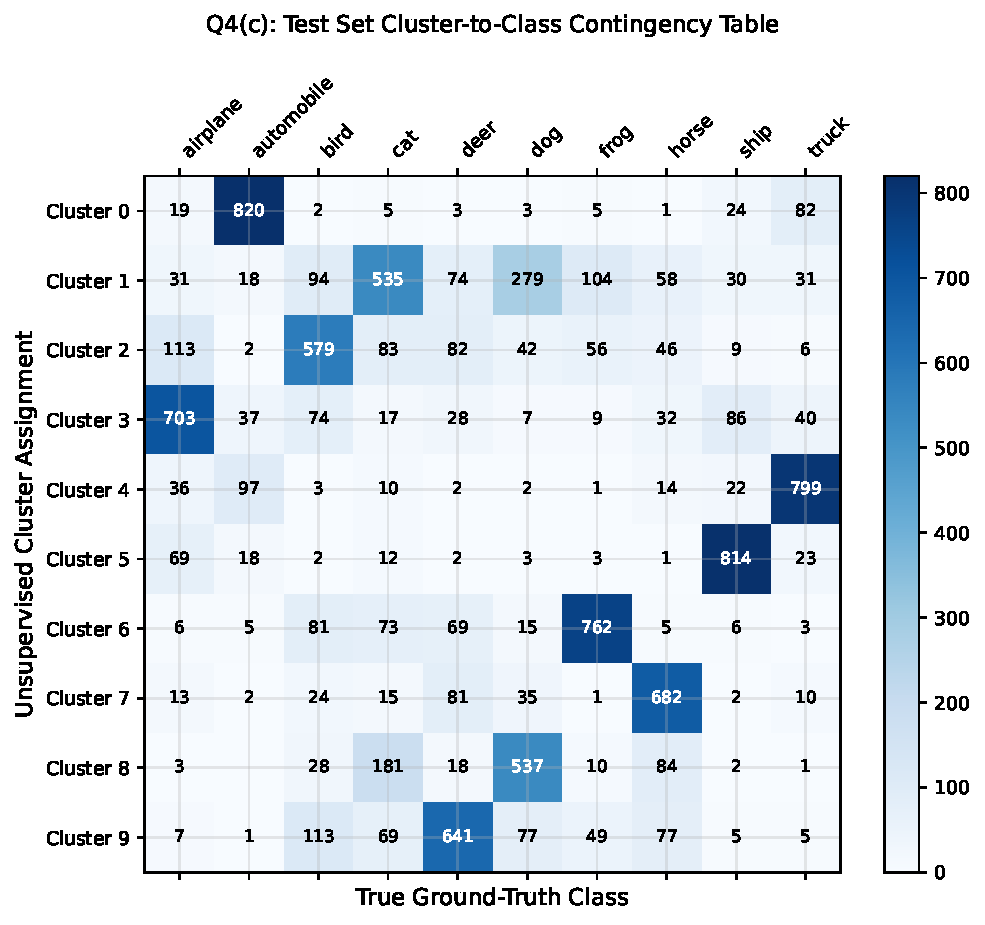
\includegraphics[width=0.48\linewidth]{figures/q4c_contingency_matrix.pdf}
\caption{Q4(c) Contingency matrix heatmap for K-Means ($K=10$) on the official CIFAR-10 test set ($N=10{,}000$).}
\label{fig:q4c_contingency}
\end{figure}

\paragraph{Quantitative Clustering Results and Exact Contingency Verification.}
Fitting $K=10$ on training representations without labels and predicting on the unblinded test set yields: K-Means ($K=10$) achieves $\text{Test ARI} = \mathbf{0.4537}, \, \text{Test NMI} = \mathbf{0.5206}$; GMM ($K=10$) achieves $\text{Test ARI} = \mathbf{0.4262}, \, \text{Test NMI} = \mathbf{0.5056}$. The recomputed contingency table (Table~\ref{tab:q4c_contingency_full} and Figure~\ref{fig:q4c_contingency}) accounts for exactly $10{,}000$ test samples ($1{,}000$ per class column), reconciling all sums.

\paragraph{Disagreement Analysis: Unsupervised Density vs. Supervised Hyperplanes.}
Contrasting unsupervised clustering against the supervised SVM ($71.64\%$) exposes fundamental geometric divergences: (1) \textit{Domestic Pet Conflation:} Cluster 1 merges $535$ cats with $279$ dogs ($1{,}254$ total), while Cluster 8 merges $537$ dogs with $181$ cats ($864$ total). Unlike the curved RBF SVM hyperplane, centroid-based clustering cannot resolve overlapping spherical quadruped manifolds without labels. (2) \textit{Environmental Conflation:} Cluster 2 merges $579$ birds and $113$ airplanes (blue-sky backgrounds); Cluster 9 merges $641$ deer and $113$ birds (green foliage). (3) \textit{Manifold vs. Margin:} Unsupervised clustering organizes by dominant ambient variance (background and pose), whereas supervised learning isolates discriminative class boundaries.
